\documentclass[a4paper, 11pt, oneside]{scrbook}

\usepackage[backend=biber]{biblatex}
\usepackage[ngerman]{babel}		
\usepackage[T1]{fontenc}	  	
\usepackage[utf8]{inputenc}
\usepackage[hidelinks]{hyperref}
\usepackage{graphicx}
\usepackage{epstopdf}
\usepackage{float}
\usepackage{microtype}
\usepackage[T1]{fontenc}
\usepackage{lmodern}
\usepackage{acronym}
\usepackage{booktabs}
\usepackage{caption}
\usepackage{csquotes}
\usepackage{url}
\usepackage{makecell}
\usepackage[table]{xcolor}
\usepackage{listings}
\usepackage{pdfpages}
\usepackage{siunitx}


% \usepackage{blindtext}

\renewcommand*{\headfont}{\normalfont}
\renewcommand*{\multicitedelim}{\addsemicolon\space}
% \renewcommand*{\headrulewidth}{0pt}
\renewcommand*{\arraystretch}{1.5}
\renewcommand*{\familydefault}{\sfdefault}

\newcommand*{\tabindent}{\hspace{3mm}}
\newcommand*{\doubletabindent}{\hspace{6mm}}

\setlength{\parskip}{1.5ex}
\lstset{numbers=left, numberstyle=\tiny, numbersep=5pt, firstnumber=1}
\lstset{language=Perl, basicstyle=\ttfamily\footnotesize,breaklines=true}

\addbibresource{bibliography.bib}
\counterwithin{figure}{section}

\begin{document}

\rowcolors{1}{white}{lightgray}

\frontmatter

\def\title{Ahead-of-Time-Compilation vs Profile-based Just in time Compilation}
\def\author{Robin Wollenschläger}

\begin{titlepage}


    \begin{minipage}[t]{0.25\textwidth}
        DHBW Mosbach\\
        Lohrtalweg 10\\
        74821 Mosbach\\
        Deutschland
    \end{minipage}
    \hfill
    \begin{minipage}[t]{0.25\textwidth}
        
\includegraphics[height=1.5cm]{prefix/image/logo-dhbw.eps}
    \end{minipage}




    \begin{center}
        \vspace{10mm}

        \huge \title

        \vspace{5mm}

        \large \bfseries Seminar Informatik an der Dualen Hochschule Baden-Württemberg Mosbach


    \end{center}

    \vspace{10mm}

    \begin{tabular}[ht]{ l p{4cm} l p{4cm} }
        Studiengang/-richtung:                               & B.Sc. - Angewandte Informatik  \tabularnewline
        Kurs:                                                & INF20B\tabularnewline
        Name, Vorname:                                       & \author \tabularnewline
        Matrikelnummer:                                      & 9495107\tabularnewline
        % Geburtsdatum:                                        & 23.07.1994\tabularnewline
        % Geburtsort:                                          & Buchen\tabularnewline
        % Name, Vorname des betrieblich Prüfenden/Betreuenden: & Bäuerle Udo \tabularnewline
        % Name, Vorname des betrieblich Prüfenden/Betreuenden: & Balagula Ilja \tabularnewline
        Name, Vorname des wiss. Prüfenden/Betreuenden:       & Prof. Dr. A. Auch \tabularnewline
        Name und Sitz des Ausbildungsbetriebes:              & GÖTTFERT Werkstoff-Prüfmaschinen GmbH \tabularnewline
                                                             & Siemensstrasse 2, 74722 Buchen \tabularnewline
        Abgabedatum:                                         & \today \tabularnewline
    \end{tabular}

    % \chapter*{Sperrvermerk}
    % \thispagestyle{empty}
    % Der Inhalt dieser Arbeit darf weder als Ganzes noch in Auszügen Personen außerhalb des Prüfungsprozesses und des  Evaluationsverfahrens zugänglich gemacht werden, sofern keine anders lautende Genehmigung der Ausbildungsstätte vorliegt.

    % \chapter*{Anmerkung Bilder/Screenshots}
    % Bilder und Screenshots in dieser Arbeit wurden bewusst ohne Daten erstellt, um den datenschutzrechtlichen Bestimmungen zu entsprechen. Falls dies nicht möglich war, wurden Bereiche mit personenbezogenen Daten geschwärzt.

    \chapter*{Ehrenw\"ortliche Erkl\"arung}

    \thispagestyle{empty}
    Ich versichere hiermit, dass ich diese Arbeit selbstständig verfasst und keine anderen als die angegebenen Quellen und Hilfsmittel benutzt habe. \\
    Ich versichere zudem, dass die eingereichte elektronische Fassung mit der gedruckten Fassung übereinstimmt.\\
    \\
    Buchen, \today
    \newpage
    \vspace{5mm}

    % \fancypagestyle{empty}{
    %   \fancyhf{}
    %   \fancyfoot[C]{\today}
    % }

\end{titlepage}


\chapter*{Abkürzungsverzeichnis}
\begin{acronym}[.NET-Framework]
    % \acro{SPS}[SPS]{Speicherprogrammierbare Steuerung}
    
\end{acronym}

\listoffigures 

\listoftables

\tableofcontents

\mainmatter

\chapter{Abstract}

\section{Deutsch}

\clearpage

\section{English}

% \input{chapters/chapter1_Einordnung.tex}
% \input{chapters/chapter2_Einleitung.tex}
% \input{chapters/chapter3_Planung.tex}
% \input{chapters/chapter4_Durchfuehrung.tex}
% \input{chapters/chapter5_Test.tex}
% \input{chapters/chapter6_Abnahme.tex}
% \input{chapters/chapter7_Auswertung.tex}
% \input{chapters/chapter8_Fazit.tex}

%\blinddocument

% \nocite{*}

\appendix
\setcounter{chapter}{23}
\chapter{Anhang}
\pagenumbering{Roman}

% \section{Basis Kapillarrheometer}
% Quelle: GÖTTFERT Werkstoff-Prüfmaschinen GmbH
% \begin{figure}[ht]
%     \begin{center}
%         \includegraphics[width=0.75\textwidth]{assets/img/DE_IMG_Prinzip_Kapillarrheometer.png}
%         \caption{Basis Kapillarrheometer}
%         \label{base_capillary_rheometer}
%     \end{center}
% \end{figure}
% \clearpage



% % \section{Detaillierte Zeitplanung nach Phasen}
% \begin{table}[ht]
%     \begin{center}
%         \begin{tabular}{| l | r  r |}
%             \hline
%             \textbf{Projektphase}                                & \multicolumn{2}{ c |}{\textbf{Zeit in h}}                \\
%             \hline

%             \textbf{Planungsphase}                               &                                           & \textbf{80} \\
%             \hline
%             \tabindent{IST-Analyse}                              & 20                                        &              \\
%             \hline
%             \tabindent{SOLL-Konzept}                             & 20                                        &              \\
%             \hline
%             \tabindent{Ablaufplanung}                            & 20                                        &              \\
%             \hline
%             \tabindent{Zeit- und Ressourcenplanung}              & 20                                        &              \\
%             \hline

%             \textbf{Durchführung}                                &                                           & \textbf{280} \\
%             \hline
%             \tabindent{Automation Mess- und Kalibrierprozess}    &                                           & 160          \\
%             \hline
%             \doubletabindent{Ablauf Temperaturmessung}           & 80                                       &              \\
%             \hline
%             \doubletabindent{Datenspeicherung}                   & 80                                        &              \\
%             \hline
%             \tabindent{Datentransfer und Auswertung}             &                                           & 120          \\
%             \hline
%             \doubletabindent{Datentransfer}                      & 40                                        &              \\
%             \hline
%             \doubletabindent{Integration PowerTool}              & 40                                        &              \\
%             \hline
%             \doubletabindent{Ermittlung Korrekturwert}           & 20                                        &              \\
%             \hline
%             \doubletabindent{Erstellung Prozessprotokoll}        & 20                                        &              \\
%             \hline

%             \textbf{Testphase/Abnahme}                           &                                           & \textbf{40}  \\
%             \hline
%             \tabindent{Testen einzelner Komponenten}             & 16                                        &              \\
%             \hline
%             \tabindent{Testen im Livebetrieb}                    & 16                                         &              \\
%             \hline
%             \tabindent{Abnahme durch Projektteam}                & 8                                        &              \\
%             \hline

%             \textbf{Auswertung/Fazit/Dokumentation}              &                                           & \textbf{80} \\
%             \hline
%             \tabindent{Auswertung: Gewinn durch Automatisierung} & 8                                        &              \\
%             \hline
%             \tabindent{Projekt-Dokumentation}                    & 72                                        &              \\

%             \hline \hline
%             \textbf{Gesamt}                                      &                                           & \textbf{480} \\
%             \hline
%         \end{tabular}
%     \end{center}
%     \caption{Detaillierte Zeitplanung nach Phasen}
%     \label{zeitplanung-detail}
% \end{table}
% \clearpage

\section{Arduino Uno R3 Datasheet}\label{arduino_datasheet}
\cite[Arduino, Webseite abgerufen am 20.12.2022]{arduino_datasheet}
% Quelle: GÖTTFERT Werkstoff-Prüfmaschinen GmbH
%  \begin{figure}[ht]
%     \begin{center}
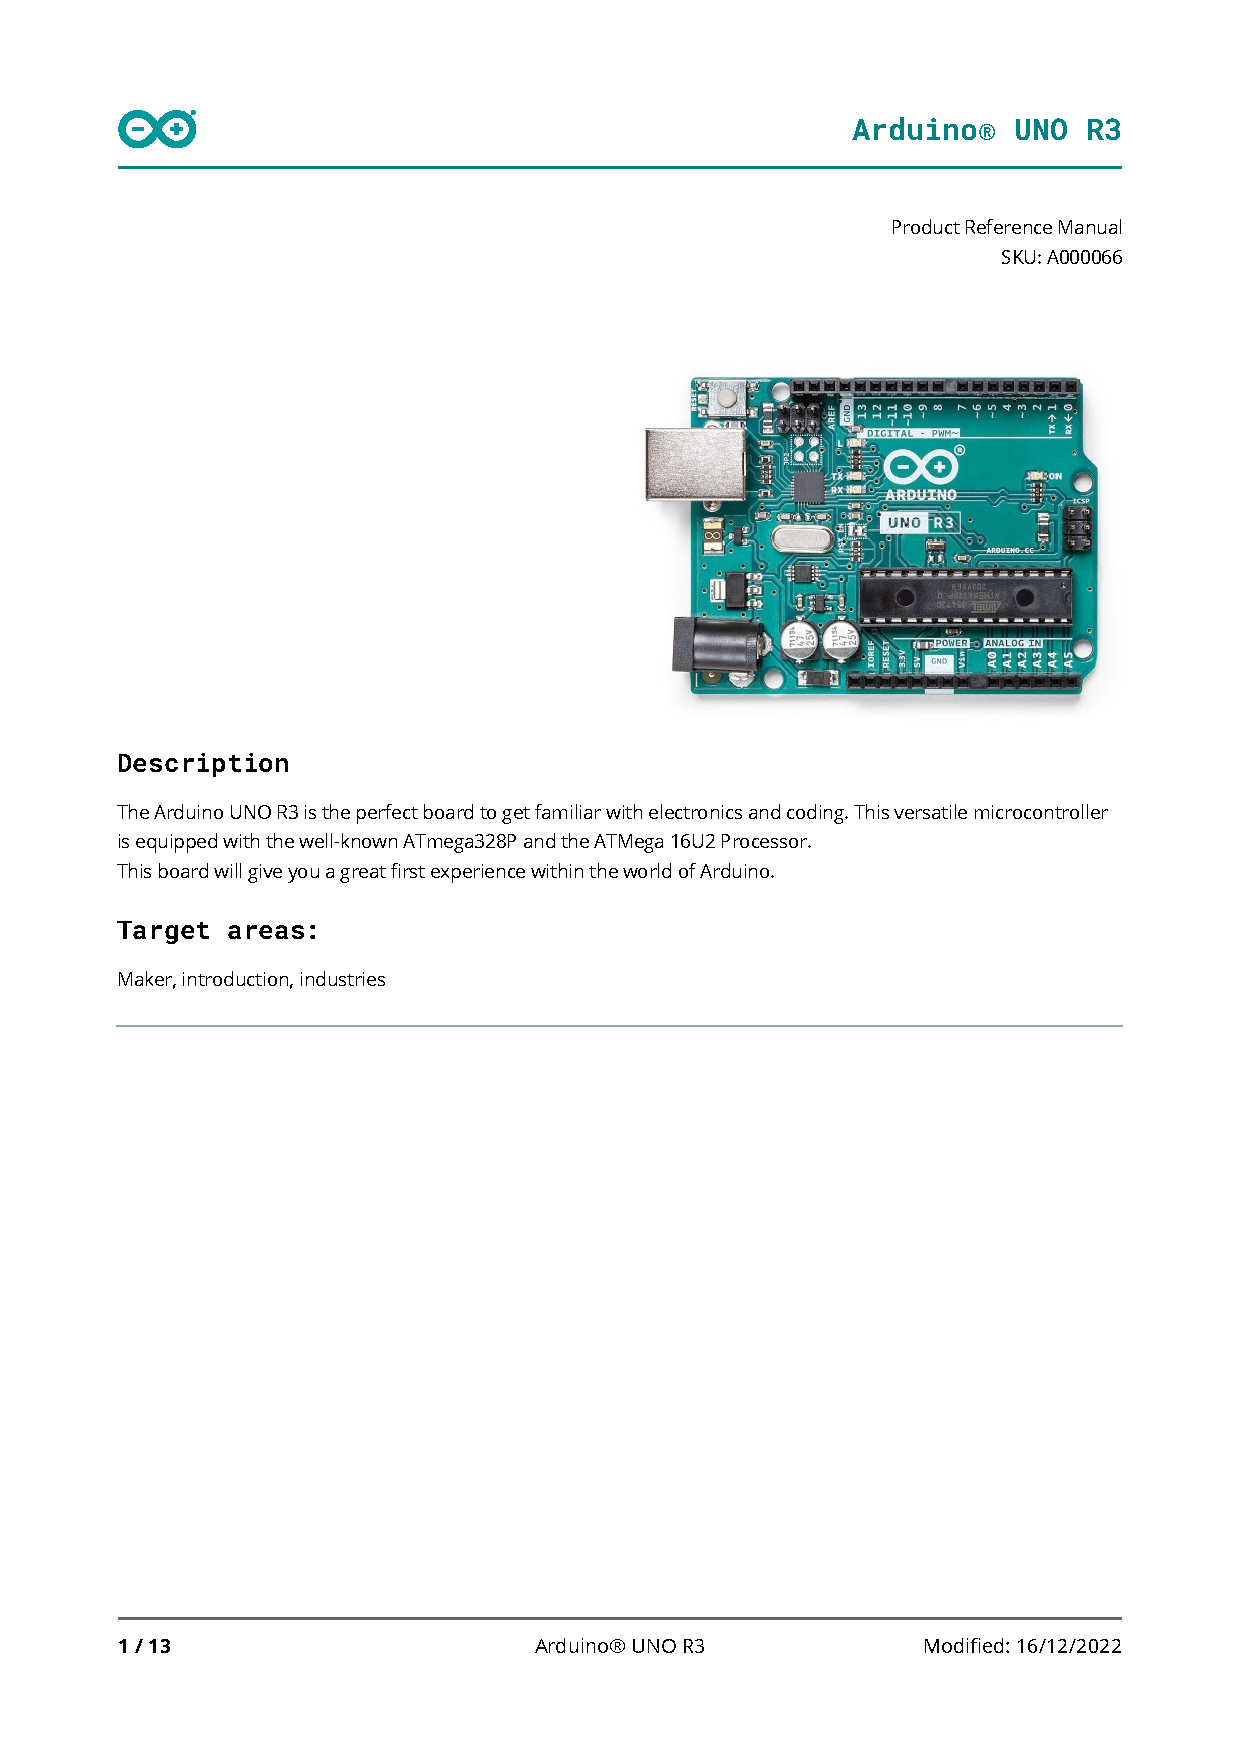
\includepdf[pages=-, landscape=true]{assets/doc/A000066-datasheet.pdf}

% %  \includegraphics[width=1.4\textwidth, angle=90]{assets/pdf/012.06.0.04.628.0_DOKU.pdf}
% %  \caption{Zeichnung Heißkanal RHEOGRAPH}

% %     \end{center}
% %  \end{figure}
% \clearpage


\backmatter

\sloppy

\printbibliography

\end{document}